\usetikzlibrary{arrows}
\usetikzlibrary{decorations.markings}
\usetikzlibrary{patterns}
%
%
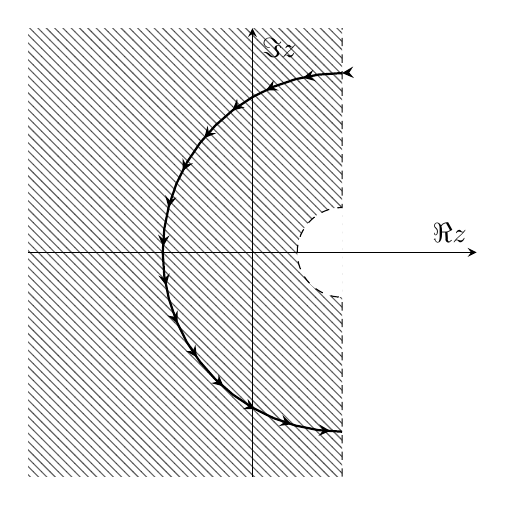
\begin{tikzpicture}
	\begin{axis} [
		axis on top,
		axis lines=middle,
		xmin=-5,
		xmax=5,
		ymin=-5,
		ymax=5,
		unit vector ratio=1 1 1,
		ticks=none,
		xlabel={$\Re z$},
		ylabel={$\Im z$}]
%
		\fill[pattern=north west lines, opacity=0.6] (-5,5) rectangle (2,-5);
		\fill[white] (2, -1) -- (2, 1) arc(90:270:1) -- cycle;
		\draw[dashed] (2, -5) -- (2, -1) arc(270:90:1) -- (2,5);
%
%
		\begin{scope}[decoration={
			markings,
			mark=between positions 0 and 1 step 5mm with {\arrow {stealth}}}]
%
			\draw [thick, postaction=decorate] plot [domain=1:3, variable=\t] ({2 + 4*cos(\t * pi / 2 r)}, {4*sin(\t * pi / 2 r)});
		\end{scope}
	\end{axis}
\end{tikzpicture}
%
